%-------------------------------------------------------------------------------
%	PACKAGES AND THEMES
%-------------------------------------------------------------------------------
\documentclass[xcolor=dvipsnames]{beamer}
\mode<presentation> {}
% The Beamer class comes with a number of default slide themes
% which change the colors and layouts of slides. Below this is a list
% of all the themes, uncomment each in turn to see what they look like.
%\usetheme{default}
%\usetheme{AnnArbor}
\usetheme{Antibes}
%\usetheme{Bergen}
%\usetheme{Berkeley}
%\usetheme{Berlin}
%\usetheme{Boadilla}
%\usetheme{CambridgeUS}
%\usetheme{Copenhagen}
%\usetheme{Darmstadt}
%\usetheme{Dresden}
%\usetheme{Frankfurt}
%\usetheme{Goettingen}
%\usetheme{Hannover}
%\usetheme{Ilmenau}
%\usetheme{JuanLesPins}
%\usetheme{Luebeck}
%\usetheme{Madrid}
%\usetheme{Malmoe}
%\usetheme{Marburg}
%\usetheme{Montpellier}
%\usetheme{PaloAlto}
%\usetheme{Pittsburgh}
%\usetheme{Rochester}
%\usetheme{Singapore}
%\usetheme{Szeged}
%\usetheme{Warsaw}
\usepackage{blkarray}
\usepackage{amsmath}
\usepackage{graphicx}
\usepackage{xfrac}
%\usepackage{xcolor}
\usepackage{listings}
%\usepackage{kbordermatrix}

\definecolor{alt}{rgb}{0.44,0.00,0.16} % SET THIS TO A WARM RED WITH RGB VALUES
%\setbeamercolor{alerted text}{fg=alt,bg=}
\usepackage[usenames,dvipsnames]{color}    

\lstset{ 
  language=R,                     % the language of the code
  basicstyle=\tiny\ttfamily, % the size of the fonts that are used for the code
  numbers=left,                   % where to put the line-numbers
  numberstyle=\tiny\color{Blue},  % the style that is used for the line-numbers
  stepnumber=1,                   % the step between two line-numbers. If it is 1, each line
                                  % will be numbered
  numbersep=5pt,                  % how far the line-numbers are from the code
  backgroundcolor=\color{white},  % choose the background color. You must add \usepackage{color}
  showspaces=false,               % show spaces adding particular underscores
  showstringspaces=false,         % underline spaces within strings
  showtabs=false,                 % show tabs within strings adding particular underscores
  frame=single,                   % adds a frame around the code
  rulecolor=\color{black},        % if not set, the frame-color may be changed on line-breaks within not-black text (e.g. commens (green here))
  tabsize=2,                      % sets default tabsize to 2 spaces
  captionpos=b,                   % sets the caption-position to bottom
  breaklines=true,                % sets automatic line breaking
  breakatwhitespace=false,        % sets if automatic breaks should only happen at whitespace
  keywordstyle=\color{RoyalBlue},      % keyword style
  commentstyle=\color{YellowGreen},   % comment style
  stringstyle=\color{ForestGreen}      % string literal style
}

\setbeamercolor{alerted text}{fg=purple,bg=}

\AtBeginSection{\frame{\tableofcontents[currentsection]}}

\graphicspath{ {img/} }		% Images live here

\title[Lord's Paradox]{Lord's Paradox}

\author{JCSzamosi}
\institute[FMF]{McMaster University Farncombe Metagenomics Facility}

\date{\today}
\begin{document}

%\begin{withoutheadline}
\begin{frame}
\titlepage
\end{frame}

\begin{frame}[plain]
\tableofcontents
\end{frame}
%\end{withoutheadline}

\section{Lord's Formulation}
\begin{frame}
``A large university is interested in investigating the effects on the students
of the diet provided in the university dining halls and any sex differences in
these effects. Various types of data are gathered. In particular, the weight of
each student at the time of his arrival in September and his weight the
following June are recorded.'' (Lord 1967, p. 304)
\end{frame}

\section{Mediation}
\begin{frame}
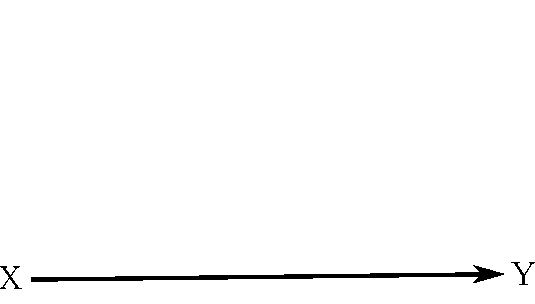
\includegraphics{arrow_diag_1.pdf}
\end{frame}

\begin{frame}{}
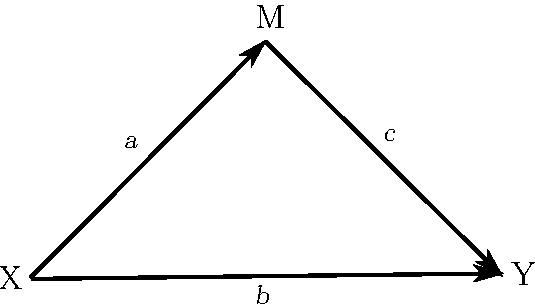
\includegraphics{arrow_diag_2.pdf}
\end{frame}

\begin{frame}{}
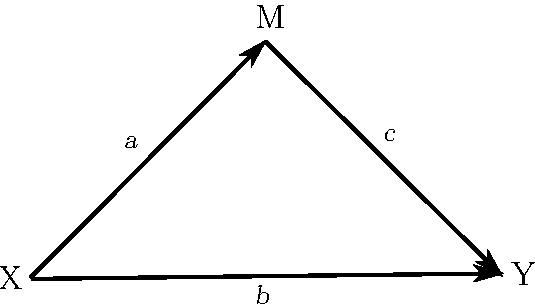
\includegraphics{arrow_diag_2.pdf}
\begin{itemize}
	\item \textbf{Total Effect} of X on Y includes the portion of the effect
	mediated by M
	\item \textbf{Direct Effect} is only the part that is \textit{not} mediated
	by M
\end{itemize} 
\end{frame}

\begin{frame}{}
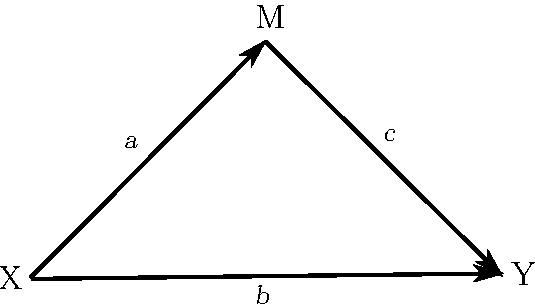
\includegraphics{arrow_diag_2.pdf}
\begin{itemize}
	\item \textbf{Total Effect} 
	\begin{itemize} 
		\item $TE = (b + ac) - a$ 
		\item $TE = b - a(1	- c)$
	\end{itemize}
	\item \textbf{Direct Effect}
	\begin{itemize} 
		\item $DE = b$
	\end{itemize} 
\end{itemize} 
\end{frame}

\subsection{Construct a mediated data set}
\begin{frame}{}
	Return to sex, initial weight, and weight gain.
	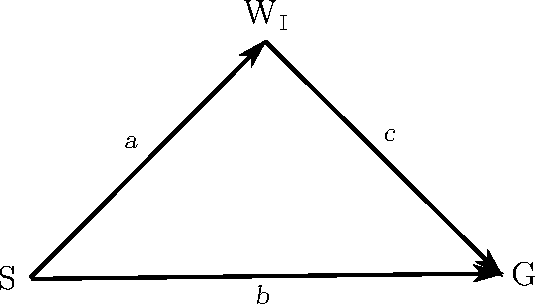
\includegraphics{arrow_diag.pdf}

	Let's construct a data set where $b = 0$, so the effect of sex on gain is
	100\% mediated by initial weight.
\end{frame}

\begin{frame}
	\begin{lstlisting}
		
		wif = rnorm(500, 150, 5)
		wim = rnorm(500, 160, 5)

		wff = (1.2 * wif) + rnorm(500, 0, 1)
		wfm = (1.2 * wim) + rnorm(500, 0, 1)

		df = data.frame(Sex = rep(c('F', 'M'), each = 500),
						Initial = c(wif, wim),
						Final = c(wff, wfm),
						Gain = c(wff - wif, wfm - wim))
	\end{lstlisting}
\end{frame} 

\end{document}
